\documentclass[11pt,a4paper]{article}
\usepackage{amsmath}
\usepackage{amssymb}
\usepackage{graphicx}
\usepackage{subfigure}
\usepackage{float}
\usepackage{xeCJK}
\usepackage{geometry}
\geometry{left=2.0cm,right=2.0cm,top=2.0cm,bottom=2.0cm}

\usepackage[T1]{fontenc}
\usepackage{xcolor}
\usepackage{lmodern}
\usepackage{listings}
\definecolor{mygreen}{rgb}{0,0.6,0}
\definecolor{mygray}{rgb}{0.5,0.5,0.5}
\definecolor{mymauve}{rgb}{0.58,0,0.82}

\lstset{
	basicstyle=\footnotesize,        % the size of the fonts that are used for the code
	breakatwhitespace=false,         % sets if automatic breaks should only happen at whitespace
	breaklines=false,                 % sets automatic line breaking
	captionpos=b,                    % sets the caption-position to bottom
	commentstyle=\color{mygreen},    % comment style
	extendedchars=true,              % lets you use non-ASCII characters; for 8-bits encodings only, does not work with UTF-8
	keepspaces=true,                 % keeps spaces in text, useful for keeping indentation of code (possibly needs columns=flexible)
	keywordstyle=\color{blue},       % keyword style
	language=[95]Fortran,                 % the language of the code
	numbers=left,                    % where to put the line-numbers; possible values are (none, left, right)
	numbersep=5pt,                   % how far the line-numbers are from the code
	numberstyle=\tiny\color{mygray}, % the style that is used for the line-numbers
	rulecolor=\color{black},         % if not set, the frame-color may be changed on line-breaks within not-black text (e.g. comments (green here))
	showspaces=false,                % show spaces everywhere adding particular underscores; it overrides 'showstringspaces'
	showstringspaces=false,          % underline spaces within strings only
	showtabs=false,                  % show tabs within strings adding particular underscores
	stepnumber=1,                    % the step between two line-numbers. If it's 1, each line will be numbered
	stringstyle=\color{mymauve},     % string literal style
	tabsize=4,                       % sets default tabsize to 2 spaces
	title=\lstname                   % show the filename of files
}


\title{磁面坐标下朗道流体程序的开发}
\author{任广智}
\date{\today}


\begin{document}
	
\maketitle
	
%\section{初始设置}	
%\subsection{坐标系的建立} 
%从gfile(eqdsk)中读取数据,得到磁面参数和一些磁面函数,用于构建所需要的磁场坐标系以及变量数组等。
%
%\begin{lstlisting}
%call read_gfile()
%out :
%	psirz(nr,nz)  矩形计算区域的极向磁通
%	R_(nr),Z_(nz)  矩形计算区域的R,Z坐标
%	rbbbs(nbbbs), zbbbs(nbbbs)  最外侧闭合磁面的(R,Z)
%\end{lstlisting}
%
%对获得的数据进行插值,以便接下来的使用和计算
%二维矩阵的插值暂时使用GTAW提供的方法,另一种可供选择的为Fortran source code中Toms660
%\begin{lstlisting}
%call gdata_interpolation2D()
%out : psi_func(xval,zval)
%\end{lstlisting}
%
%对于自定义的坐标系网格,我们需要处理gfile读取的数据,提取最外侧闭合磁面以内的磁面,并且通过插值等重构处我们所需要的磁面坐标。这里采用的磁面坐标为$(\psi,\theta,\phi)$保留了环向角的物理意义,$\psi$和$\theta$的物理意义可以具体地通过定义给出。其中$\nabla\phi$和$\nabla\psi$,$\nabla\theta$保持正交,而后两者不一定正交。
%
%首先需要定义径向坐标 $\psi$,径向坐标可以有多种取法,包括极向磁通和环向磁通的归一化以及变形而来
%\begin{lstlisting}
%call define_radial_coordinate()
%out :
%ra(nra)  归一化的径向坐标,自定义数组大小nra
%dra  间距大小
%dpsida(nra)  极向磁通的径向偏微分 
%\end{lstlisting}
%
%其次需要得到角向的坐标 $\theta$, $\theta$可以选择constant arc length或者straight line的形式。具体方法可以follow [Jardin 2010]上的方法以及[GTAW Huyoujun]程序。通过这种方法我们可以得到角向的坐标(需要归一化)。选择坐标形式或者$\theta$坐标
%固定$\phi$向的为环向,我们在处理过程中可以保持$\nabla\phi$与其他两个基矢的正交关系。通过选择$J_{tmp}$来设定$\theta$坐标的物理意义,包括constant arc length
%/straight line/constant area/constant volumn
%\begin{lstlisting}
%call define_theta_coordinate()
%out :
%th(nth)  归一化的极向坐标,自定义数组大小nth
%dth  间距大小 
%\end{lstlisting}
%
\subsection{平衡量表示}
雅克比的计算有两种方法,可以相互比较和对照 
$$J(\psi,\theta) = R(R_\theta Z_\psi-R_\psi Z_\theta)$$ $$J(\psi,\theta) = \oint\frac{R}{J_{tmp}|\nabla\psi|}dl_p/{2\pi} J_{tmp}$$

在定义一些微分算符之前,我们需要计算出所需要的度量张量的各个分量,这些分量在一般的矢量计算中会用到。包括 
$$J_{11} = |\nabla\psi|^2 = \frac{R^2}{J^2}(R_\theta^2 + Z_\theta^2)$$ 
$$J_{22} = |\nabla\theta|^2 = \frac{R^2}{J^2}(R_\psi^2 + Z_\psi^2)$$ $$J_{33} = |\nabla\phi|^2 = \frac{1}{R^2} $$ 
$$J_{12} = J_{21} = \nabla\theta\cdot\nabla\psi = -\frac{R^2}{J^2}(R_\psi R_\theta + Z_\psi Z_\theta) $$

现在我们可以推导一些流体方程中出现的算符和项的具体表现形式了。
磁场和磁场各个分量 :
$$ \pmb{B_0} = \nabla\times\pmb{A} $$ 
$$ \pmb{B_0} = \nabla\times(A_\phi\hat\phi) + (\frac{\partial{A_R}} {\partial{Z}}-\frac{\partial(A_Z)}{\partial{R}})\hat\phi $$ 
$$ \Psi(R,Z) = RA_\phi $$ 
$$ \pmb{B_0} = \nabla\Psi(R,Z)\times\nabla\phi+g(R,Z)\nabla\phi $$ $$ \pmb{B_p} = \nabla\Psi(R,Z)\times\nabla\phi $$ 
$$ \pmb{B_t} = g(R,Z)\nabla\phi $$ 
$$ B_R = -\frac{1}{R}\frac{\partial\Psi}{\partial{Z}} $$ 
$$ B_Z = \frac{1}{R}\frac{\partial\Psi}{\partial{R}} $$
这里$q$为local的$q$,$q = q(\psi)$只在straight field line的时候成立 
$$ 
\begin{aligned} 
q(\psi,\theta) &=\frac{\pmb{B_0}\cdot\nabla\phi}{\pmb{B_0}\cdot\nabla\theta} \\ 
&= -\frac{gJ}{\Psi'R^2} 
\end{aligned} 
$$

$$ 
\begin{aligned} 
\pmb{B_0} &= \Psi'\nabla\psi\times\nabla\phi + g(\psi)\nabla\phi \\ 
&= \Psi'[\nabla\psi\times\nabla\phi - q(\psi,\theta)\nabla\psi\times\theta] \\ 
&= (\Psi'\frac{J}{R^2}\nabla\theta\cdot\nabla\psi)\nabla\psi + (-\Psi'\frac{J}{R^2}|\nabla\psi|^2)\nabla\theta + g(\psi)\nabla\phi \end{aligned} 
$$
%
%
%
%\subsection{方程变换} 
%首先是$V_E\cdot\nabla$,这里考虑 $B_T \gg B_p$的近似,即$\pmb{B}=\pmb{B_T}=g(\psi)\nabla\phi$。但是这种假设并不是真正考虑了$k_\parallel\ll k_\perp$的结果,这一点在field aligned的坐标系下比较容易做到。所以如果是三维有限差分的话,需要考虑上$B_p$的贡献。
%
%$$
%\begin{aligned}
%V_E\cdot\nabla f
%&= -\frac{\nabla\Phi\times\pmb{B_T}}{B^2_0}\cdot\nabla f \\  
%&= \frac{1}{B_0^2}\nabla\Phi\times\nabla f\cdot g(\psi)\nabla\phi \\ 
%&= \frac{g}{JB^2_0}(\Phi_\psi f_\theta - \Phi_\theta f_\psi) \\
%&= \frac{g}{JB^2_0}[\Phi,f] 
%\end{aligned}    
%$$	
%	
%$$
%\begin{aligned}
%V_E\cdot\nabla f_0(\psi)
%&= -\frac{\nabla\Phi\times\pmb{B_T}}{B^2_0}\cdot\nabla f_0 \\
%&= -\frac{g}{JB^2_0} \Phi_\theta f_\psi
%\end{aligned}
%$$
%	
%平行微分算符$\nabla_\parallel$
%$$ 
%\nabla_\parallel f = \pmb{b_0}\cdot\nabla f = -\frac{\Psi'J^{-1}}{B_0}(f_\theta + qf_\phi)  
%$$
%	
%拉普拉斯算符$\nabla^2_\perp$,目前使用的一些基本算湍流输运的流体方程中,我们只使用了垂直磁场方向的laplace算符,同上边的对流项,这里的垂直不并不是严格意义上的垂直,而是在$(\psi,\theta)$平面的算符,严格的计算也会加入后续比较,即$\nabla^2_\perp f= \nabla^2 f - \nabla^2_\parallel f$,暂时如下计算:
%$$
%\begin{aligned}
%\nabla_\perp^2 f  
%&= \nabla\cdot(f_\psi \nabla\psi + f_\theta\nabla\theta) \\
%&= \nabla\cdot[ (f_\psi J_{11} + f_\theta J_{21}) \nabla\theta\times\nabla\phi\mathcal{J} + (f_\psi J_{12}+f_\theta J_{22}) \nabla\phi\times\nabla\psi\mathcal{J} ] \\
%&= \frac{1}{\mathcal{J}} 
%[ \frac{\partial}{\partial_\psi}\mathcal{J}(J_{11}f_\psi + J_{21}f_\theta) 
%+\frac{\partial}{\partial_\theta}\mathcal{J}(J_{12}f_\psi + J_{22}f_\theta) ]  
%\end{aligned}
%$$
%
%磁曲率项
%$$
%\begin{aligned}
%\nabla\cdot{\pmb{V_E}} 
%&= \nabla(\frac{1}{B_0^2})\cdot(\pmb{B_0}\times\nabla\Phi) \\
%&= \frac{2}{B_0^3}\nabla{B_0}\cdot(\nabla\Phi\times\pmb{B_0}) \\
%&\approx \frac{2}{B_0^2}\nabla{B_0}\times\nabla\Phi\cdot\pmb{B_T}    \\
%&= \frac{2g}{\mathcal{J}B_0^3}[B_0,\Phi]  
%\end{aligned}
%$$
%
%\section{简单的测试}
%\subsection{对流方程}
%考虑如下形式的温度对流方程
%$$ \frac{\partial T}{\partial t} + \pmb{V}\cdot\nabla T = 0$$ 
%这里取$\pmb{V} = V(\psi)\nabla\phi\times\nabla\psi J$,即取极向截面上与$\nabla\psi$垂直的方向,$\pmb{V}\cdot\nabla T = V(\psi)T_\theta $。使用欧拉法进行时间推进,二阶中心差分进行空间离散。取初始$T(\psi,\theta) = cos(\theta)exp(-(\psi-0.5)^2/0.1) $,速度$V(\psi) = 2\pi $ 。结果如下。
%
%\begin{figure}[H]
%	\centering
%	\subfigure{
%		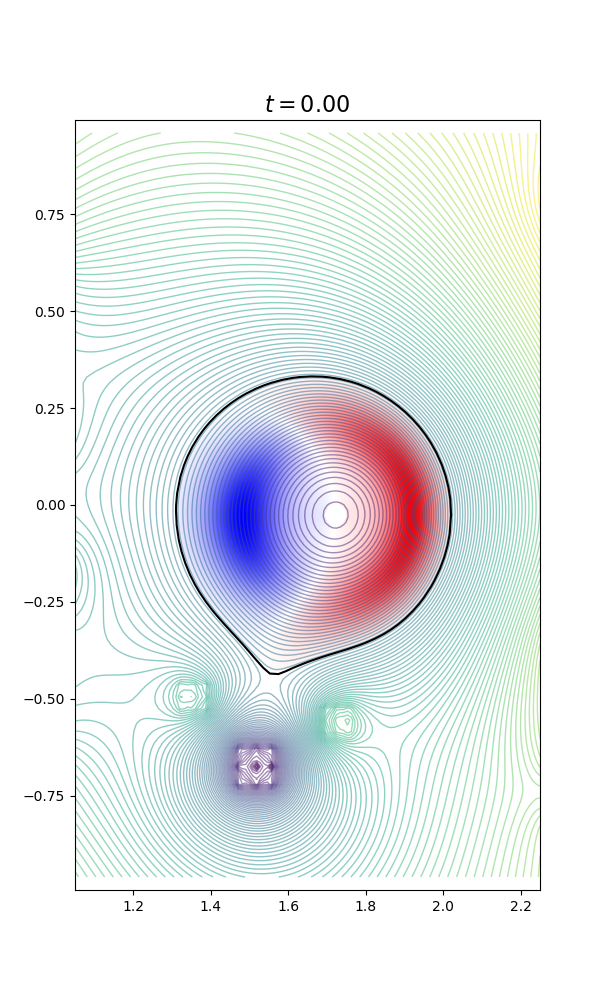
\includegraphics[width=0.15\textwidth]{../psi-code/test_01/test_01_t0.png} 
%	}
%	\subfigure{
%		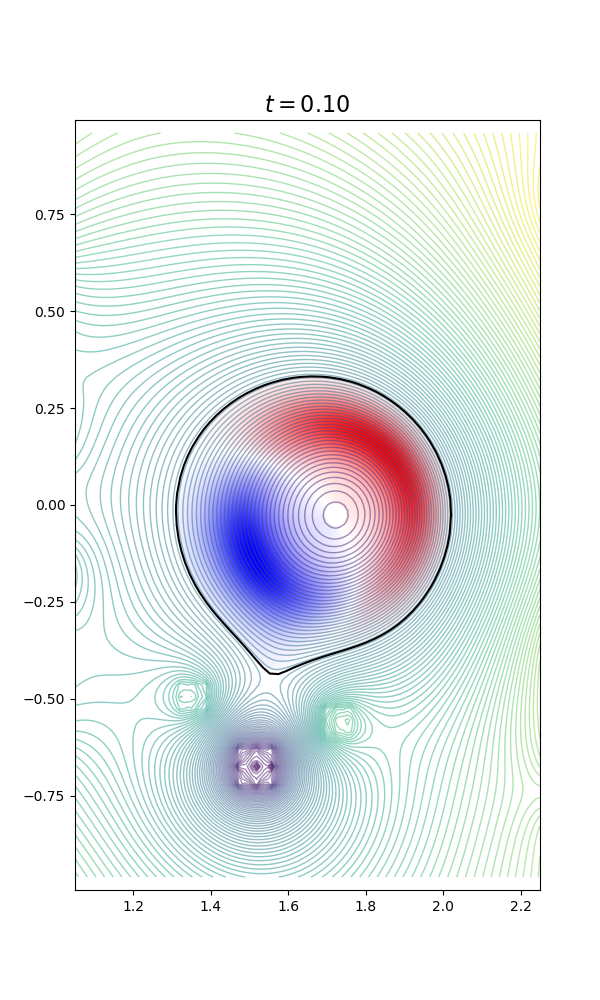
\includegraphics[width=0.15\textwidth]{../psi-code/test_01/test_01_t100.png}
%	}
%	\subfigure{
%		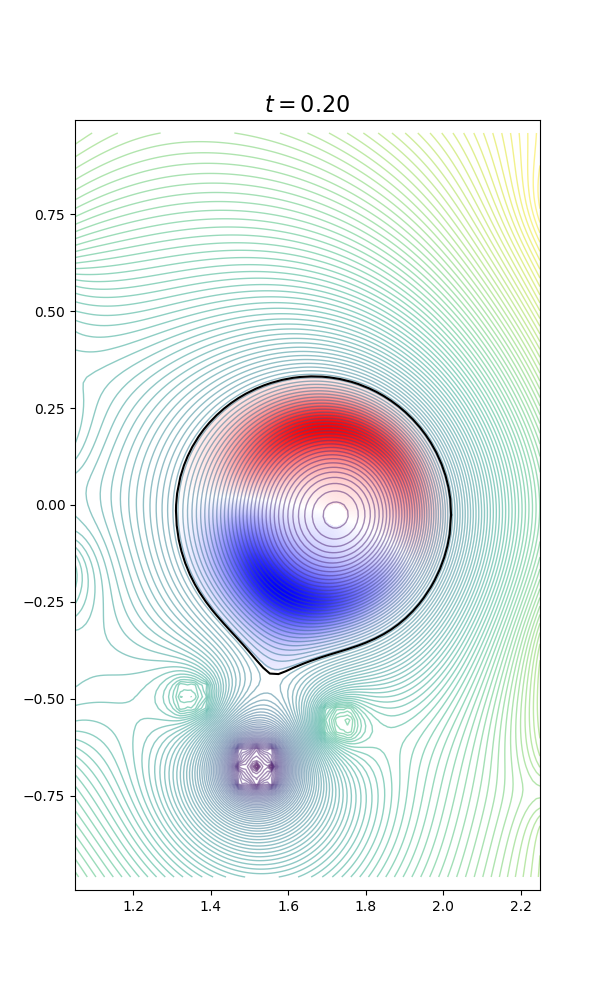
\includegraphics[width=0.15\textwidth]{../psi-code/test_01/test_01_t200.png}
%	}
%	\subfigure{
%		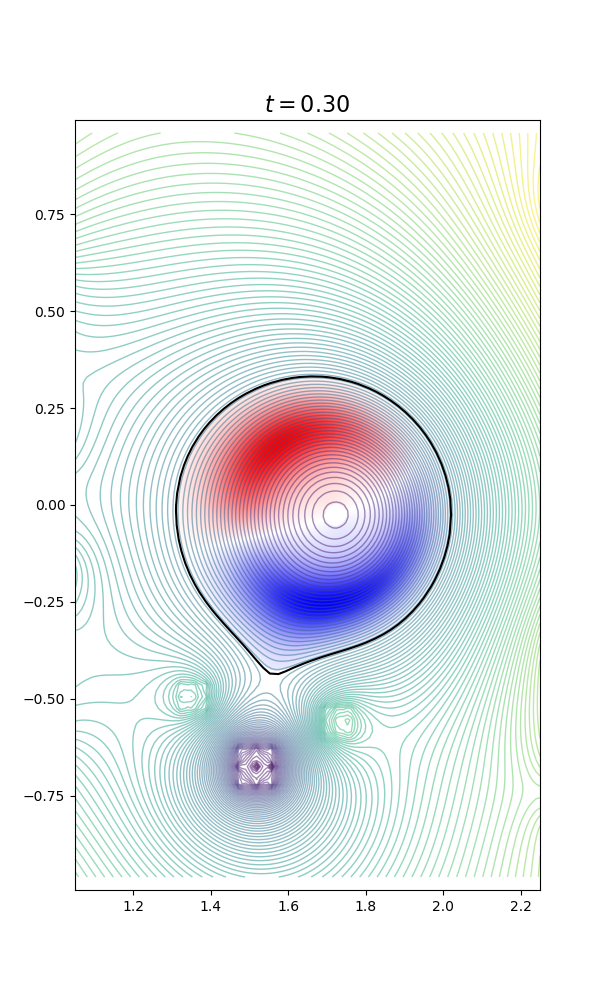
\includegraphics[width=0.15\textwidth]{../psi-code/test_01/test_01_t300.png}
%	}
%	\subfigure{
%		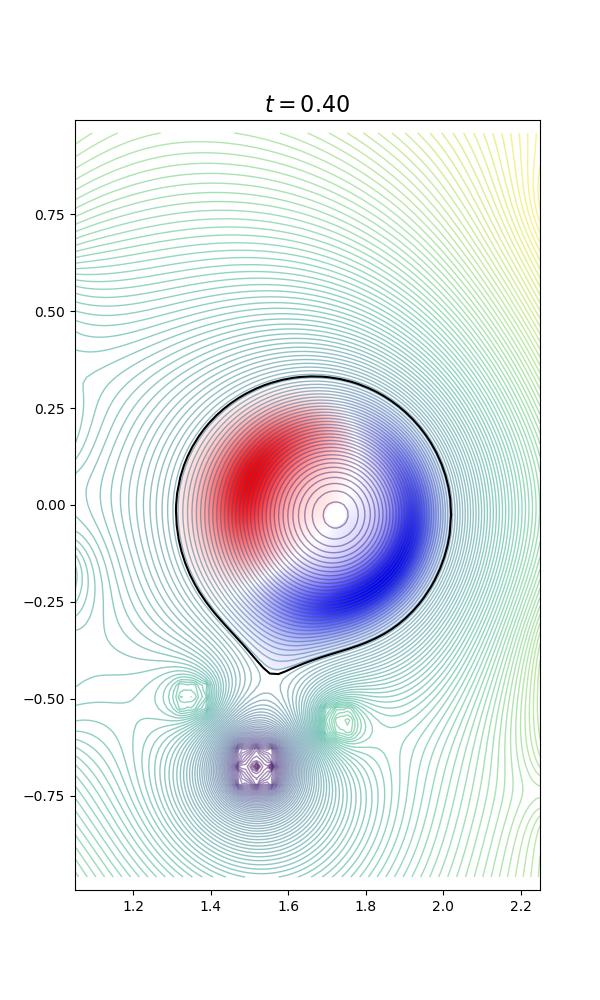
\includegraphics[width=0.15\textwidth]{../psi-code/test_01/test_01_t400.png}
%	}
%		\subfigure{
%		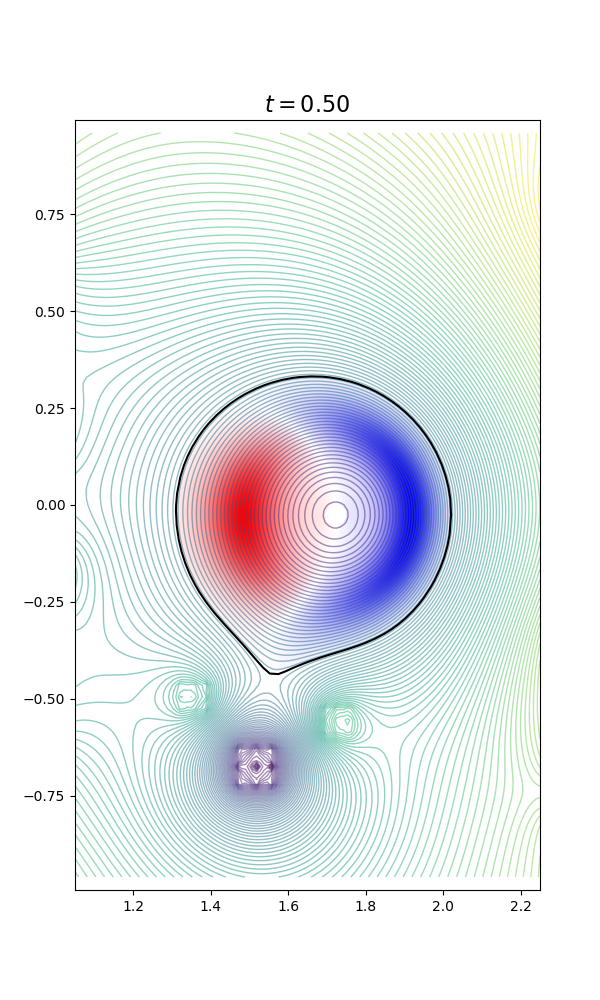
\includegraphics[width=0.15\textwidth]{../psi-code/test_01/test_01_t500.png} 
%	}
%	\subfigure{
%		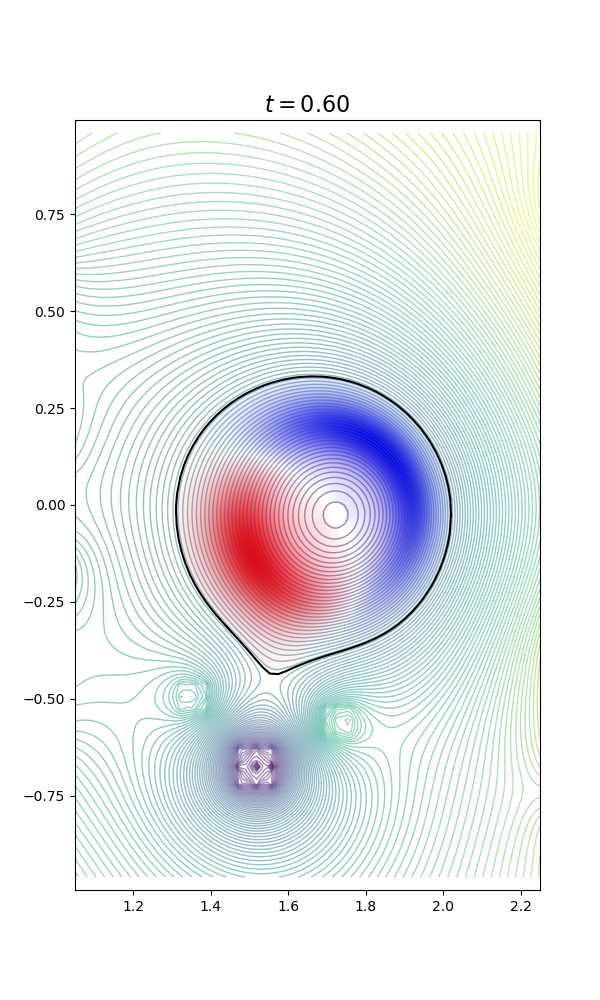
\includegraphics[width=0.15\textwidth]{../psi-code/test_01/test_01_t600.png}
%	}
%	\subfigure{
%		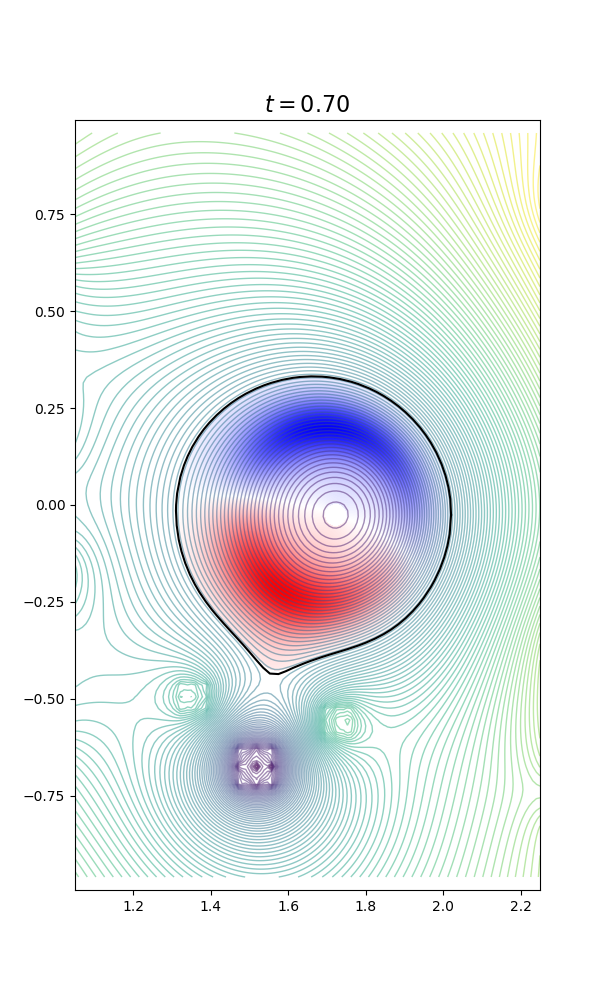
\includegraphics[width=0.15\textwidth]{../psi-code/test_01/test_01_t700.png}
%	}
%	\subfigure{
%		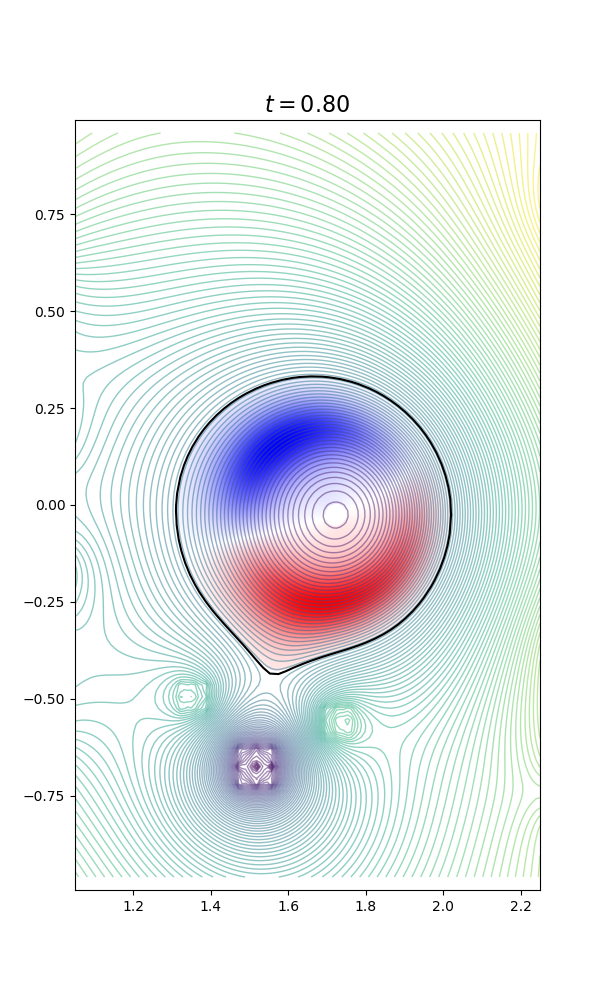
\includegraphics[width=0.15\textwidth]{../psi-code/test_01/test_01_t800.png}
%	}
%	\subfigure{
%		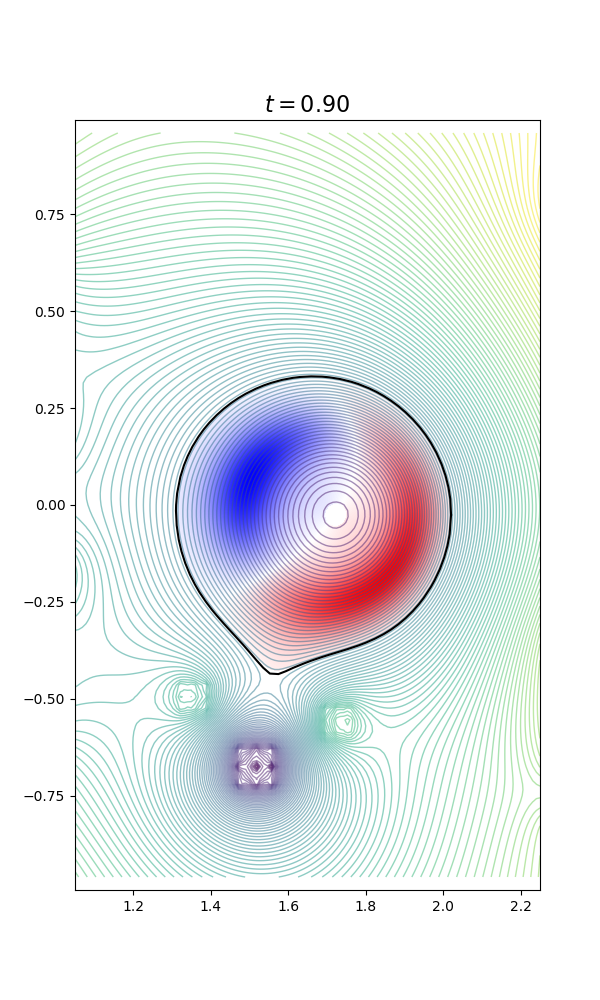
\includegraphics[width=0.15\textwidth]{../psi-code/test_01/test_01_t900.png}
%	}
%
%	\caption{}
%\end{figure}
%在托卡马克中,这里的对流主要有$\pmb{E}\times\pmb{B}$和$\nabla P\times\pmb{B}$漂移的贡献,当我们考虑磁场$B_T >> B_P$时,漂移方向即为上述的形式,实际相当于一维的问题。当考虑极向磁场时,漂移沿垂直磁场方向,并不在此时坐标系的极向截面上,这个问题待补充比较。
%
%\subsection{扩散方程}
%考虑如下形式的二维扩散方程
%$$ \frac{\partial T}{\partial t} = D\nabla_\perp^2 T $$
%这里依然假设$B_T >> B_P$
%\begin{figure}[H]
%	\centering
%	\subfigure{
%		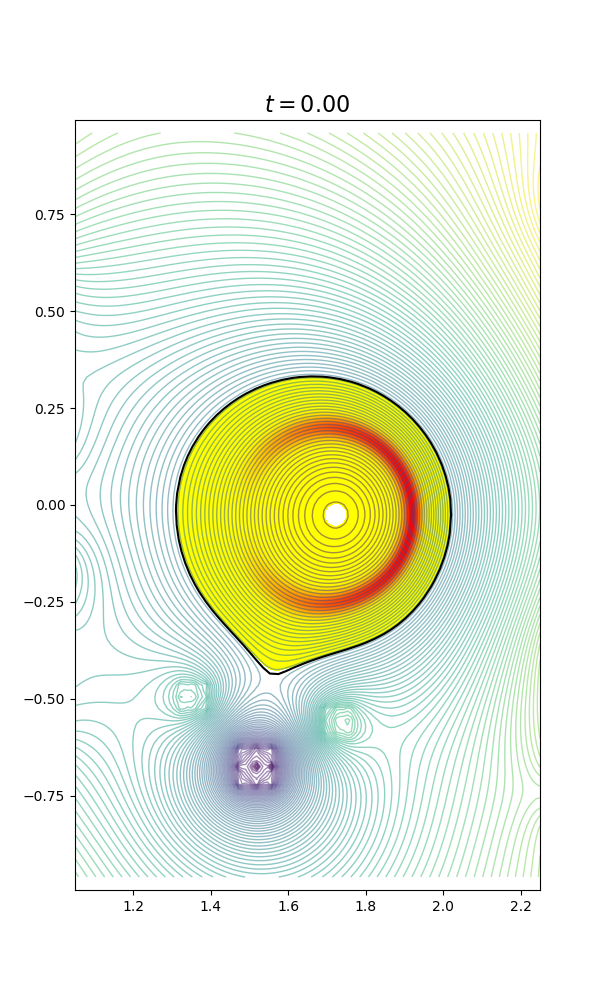
\includegraphics[width=0.15\textwidth]{../psi-code/test_02/test_02_t0.png} 
%	}
%	\subfigure{
%		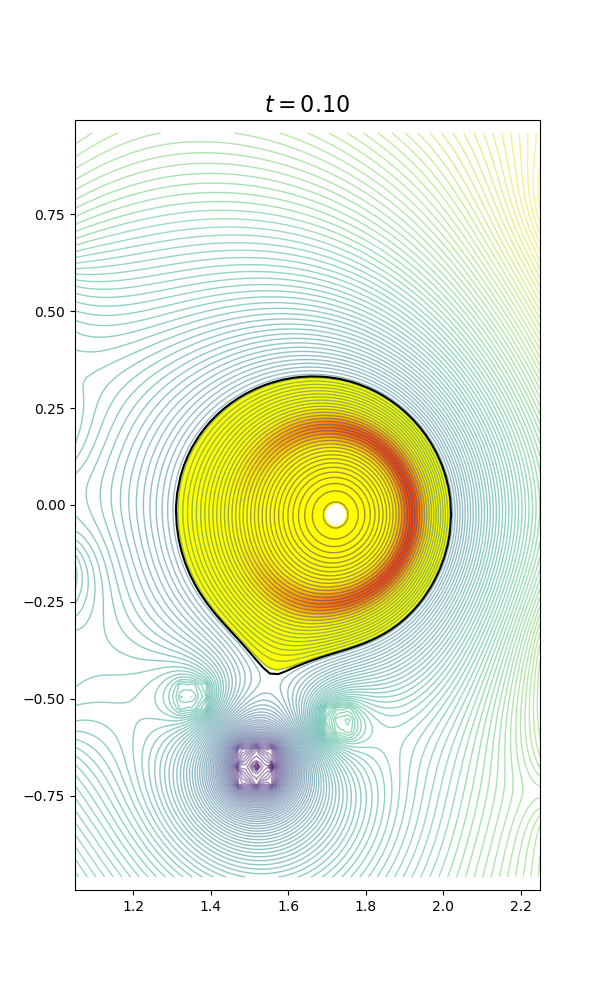
\includegraphics[width=0.15\textwidth]{../psi-code/test_02/test_02_t100.png}
%	}
%	\subfigure{
%		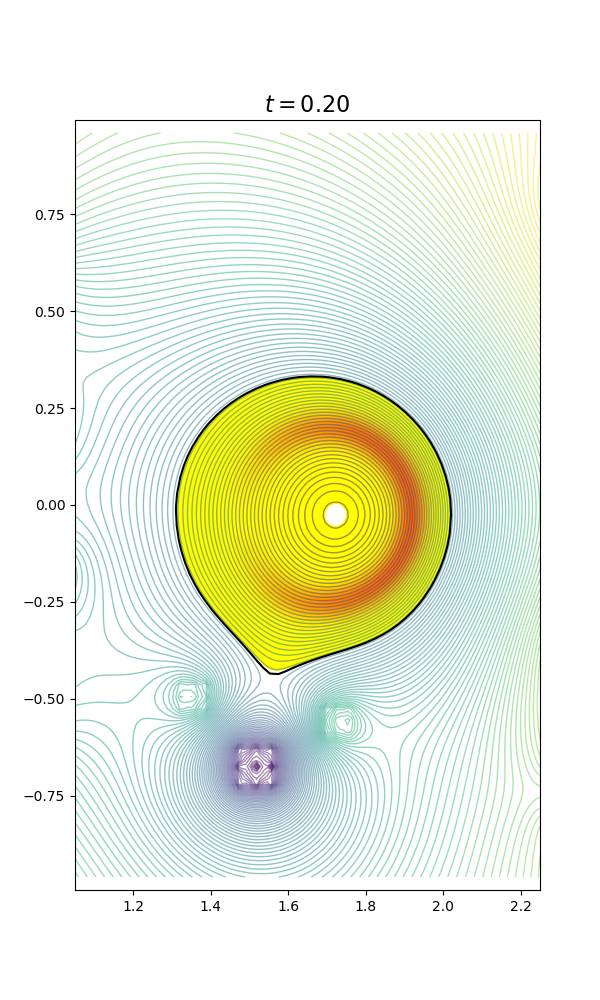
\includegraphics[width=0.15\textwidth]{../psi-code/test_02/test_02_t200.png}
%	}
%	\subfigure{
%		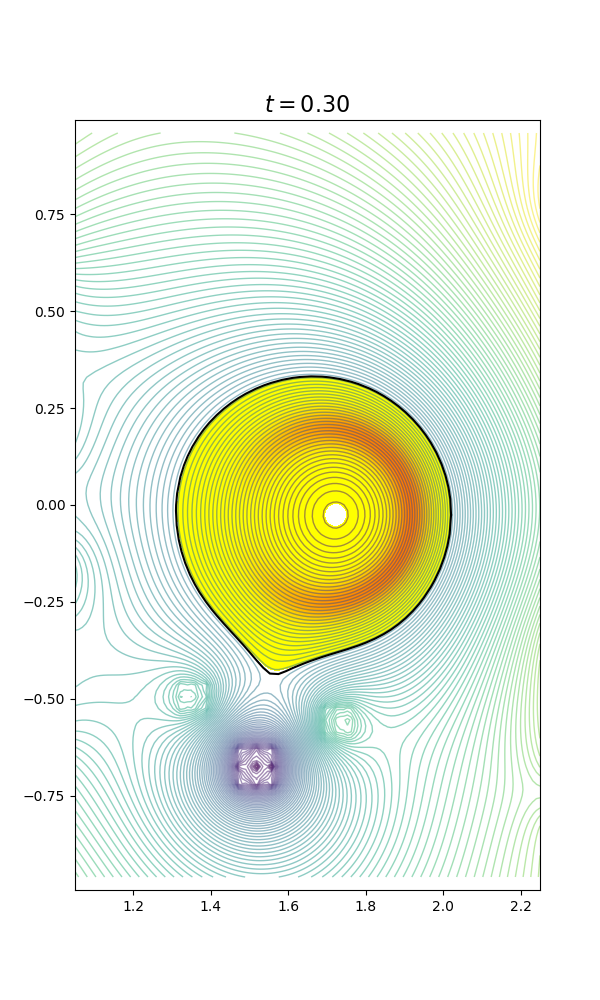
\includegraphics[width=0.15\textwidth]{../psi-code/test_02/test_02_t300.png}
%	}
%	\subfigure{
%		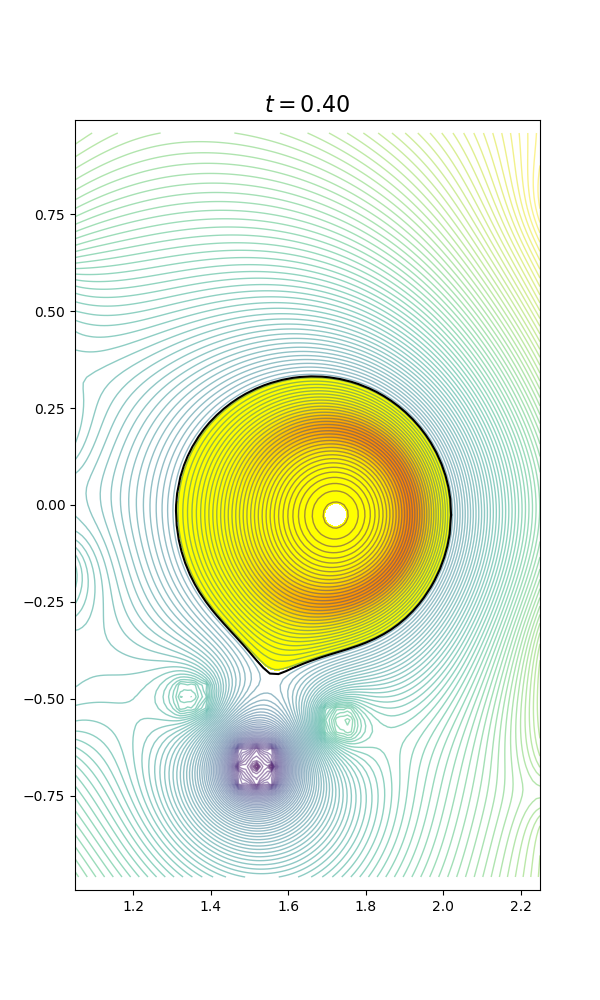
\includegraphics[width=0.15\textwidth]{../psi-code/test_02/test_02_t400.png}
%	}
%	\subfigure{
%		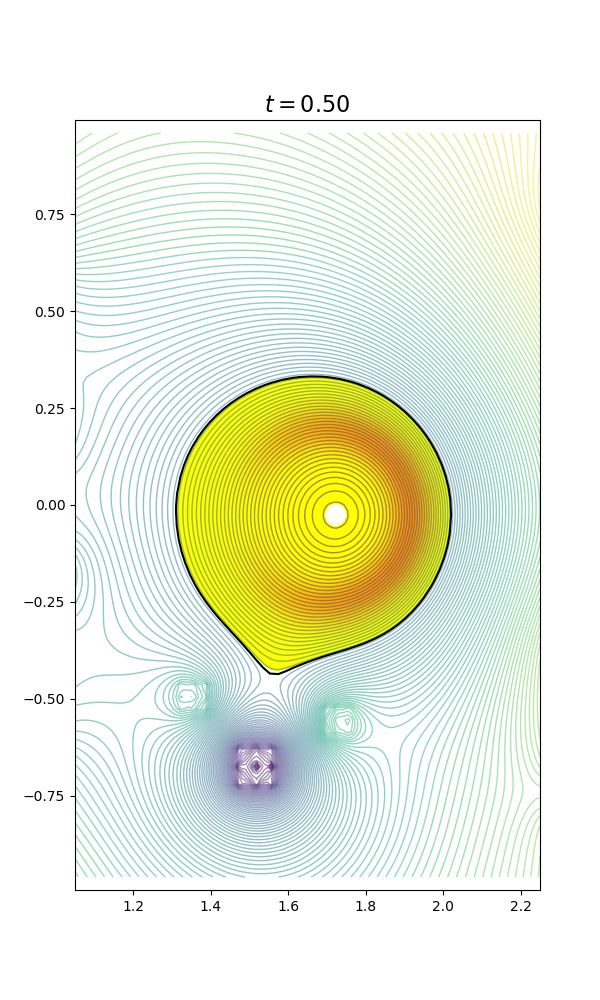
\includegraphics[width=0.15\textwidth]{../psi-code/test_02/test_02_t500.png} 
%	}
%	\subfigure{
%		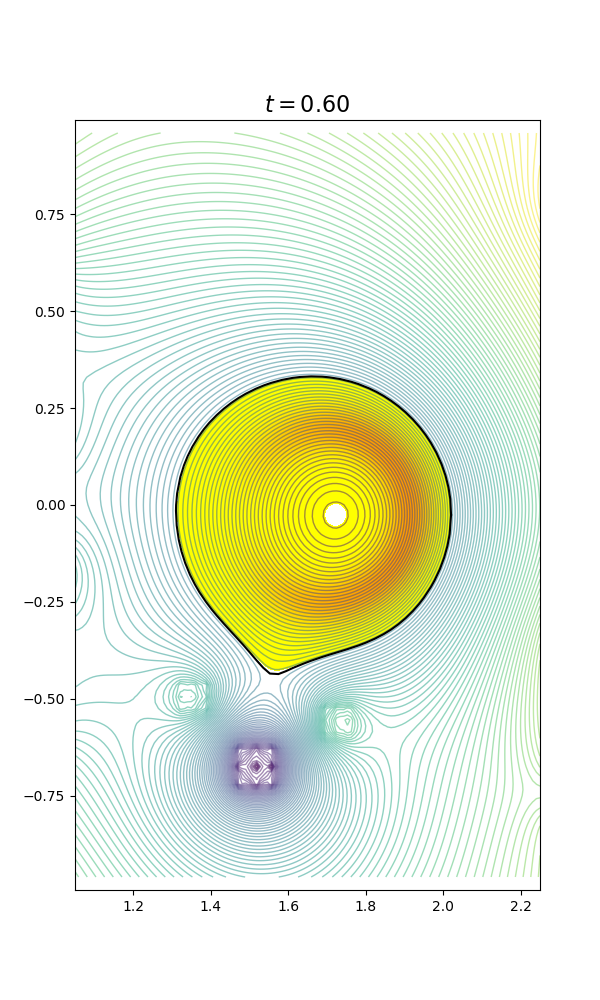
\includegraphics[width=0.15\textwidth]{../psi-code/test_02/test_02_t600.png}
%	}
%	\subfigure{
%		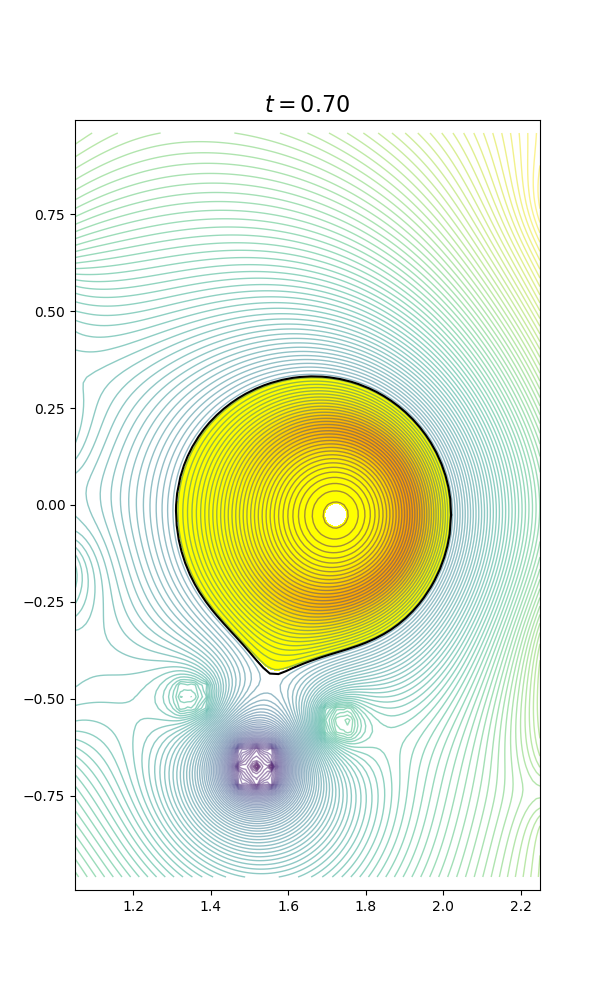
\includegraphics[width=0.15\textwidth]{../psi-code/test_02/test_02_t700.png}
%	}
%	\subfigure{
%		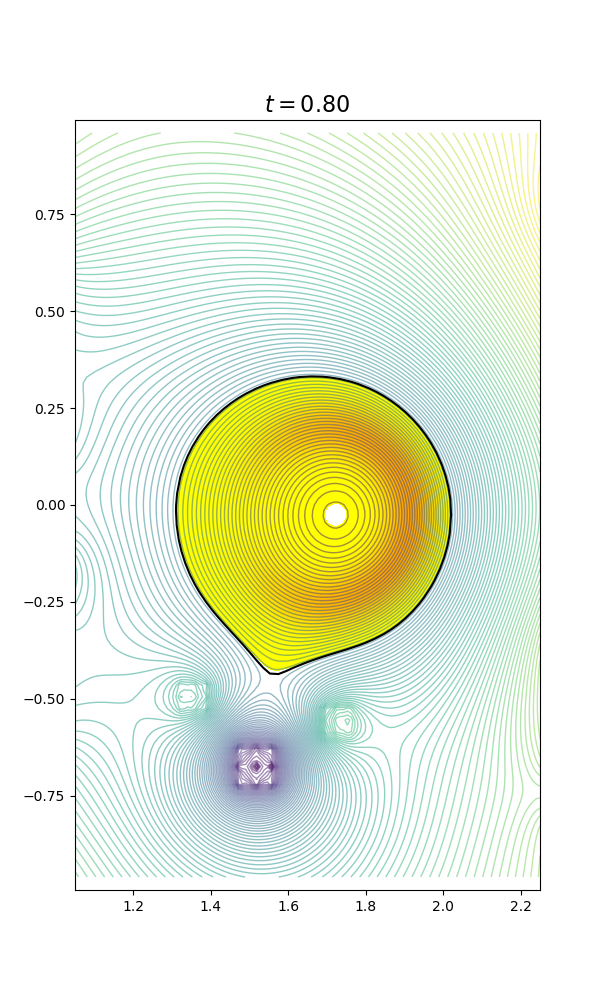
\includegraphics[width=0.15\textwidth]{../psi-code/test_02/test_02_t800.png}
%	}
%	\subfigure{
%		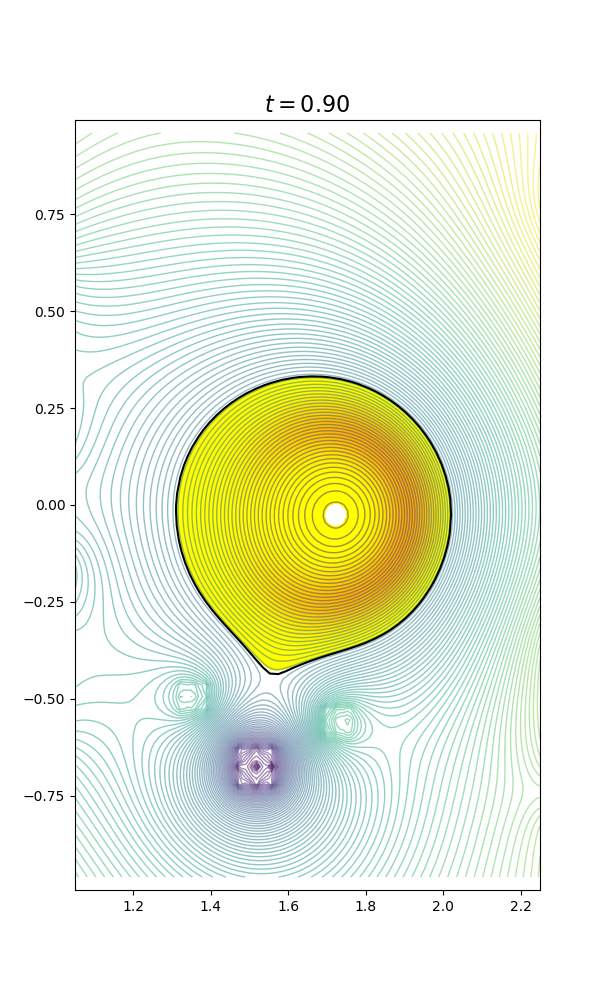
\includegraphics[width=0.15\textwidth]{../psi-code/test_02/test_02_t900.png}
%	}
%	
%	\caption{}
%\end{figure}
%
%\subsection{极向fft}
%	\begin{figure}[H]
%	\centering
%	\subfigure{
%		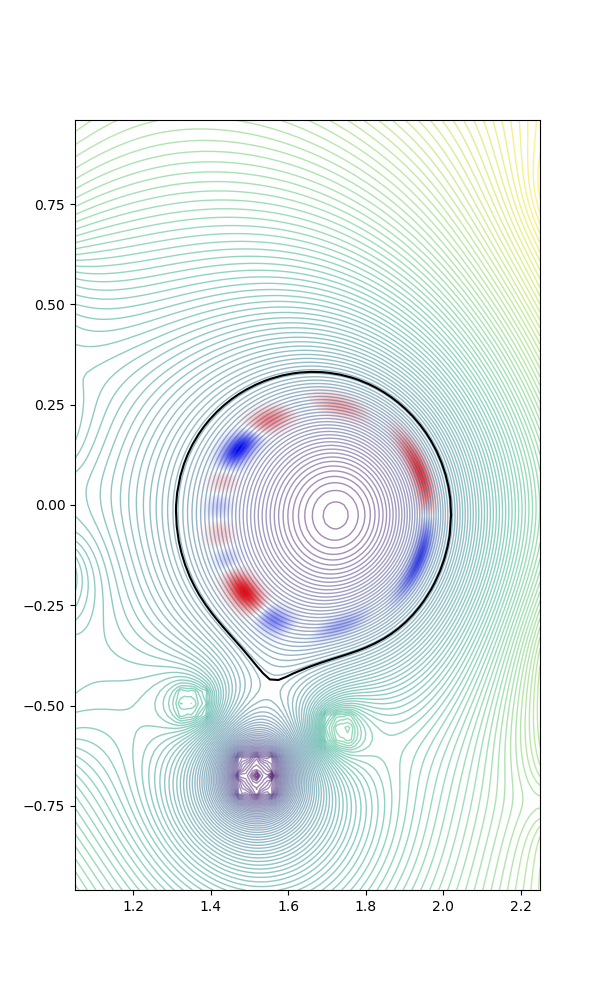
\includegraphics[width=0.15\textwidth]{../psi-code/test_03/test_03_0.png} 
%	}
%	\subfigure{
%		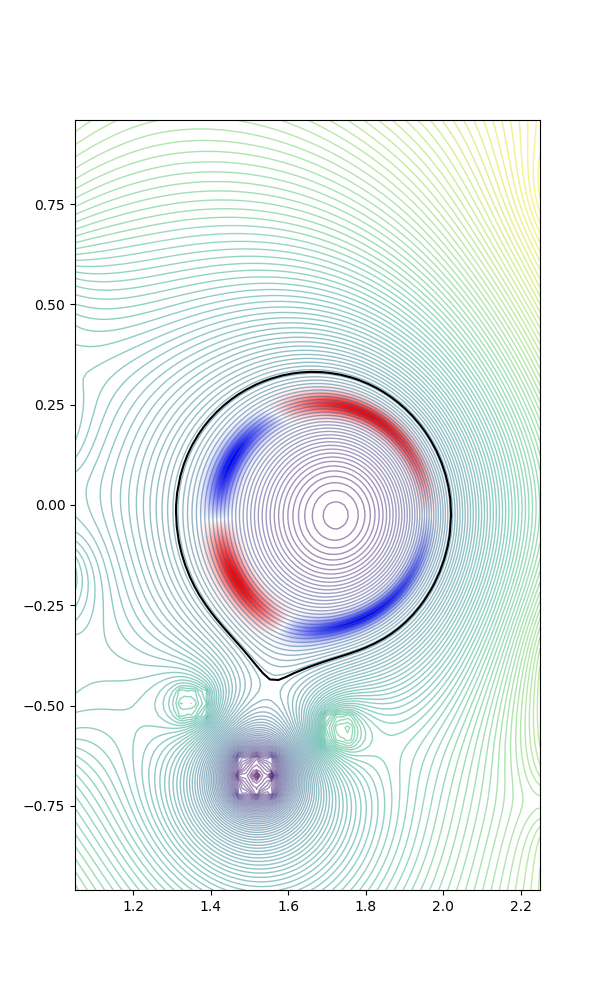
\includegraphics[width=0.15\textwidth]{../psi-code/test_03/test_03_m02.png}
%	}
%	\caption{}
%	\end{figure}
%
%\subsection{二维泊松方程}
%$$ \nabla_\perp^2 f = w $$
%$$
%\frac{\partial}{\partial_\psi}\mathcal{J}(J_{11}f_\psi + J_{21}f_\theta)+\frac{\partial}{\partial_\theta}\mathcal{J}(J_{12}f_\psi + J_{22}f_\theta) = {\mathcal{J}}w 
%$$
%直接全矩阵求解2D泊松方程,这里使用了lapack或者petsc的库来解,主要的做法就是把有限差分的系数矩阵展开成二维形式,对于二维(m,n)矩阵的解系数矩阵为(mn,mn)的尺寸,这是个很大的矩阵,在双精度下求解256X256的二维解的话需要32G的内存来存储这个系数矩阵。这个系数矩阵的元素分布如下。这里的坐标即为行和列的指标。其中除了有色的元素之外都是0元素,所以这是个稀疏的矩阵。红色的元素为径向坐标和极向坐标二阶导的元素,蓝色元素为在此基础上考虑$\theta$方向周期性条件添加的元素,绿色的元素为混合偏导带来的元素,而黑色的为混合偏导考虑$\theta$周期性边界条件添加的元素。这里的测试并未设置边界条件,也即边界条件固定为零,边界条件的进入可以通过设置右手项矩阵或者系数矩阵的方式来添加。
%\begin{figure}[H]
%	\centering
%	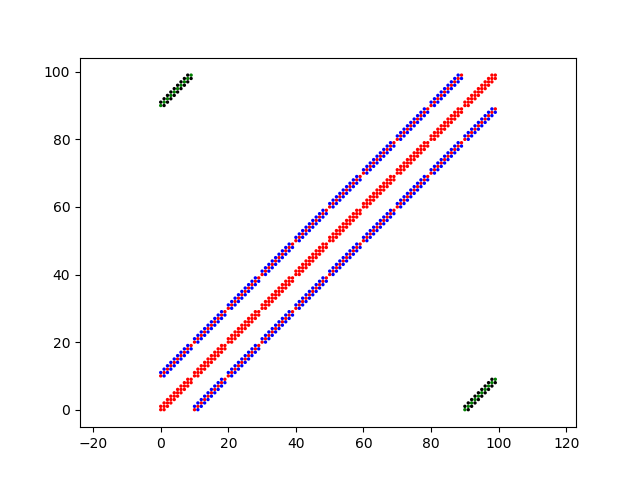
\includegraphics[width=0.4\textwidth]{../psi-code/test_06/coef.png}
%	\caption{}
%\end{figure}
%
%\begin{figure}[H]
%	\centering
%	\subfigure{
%		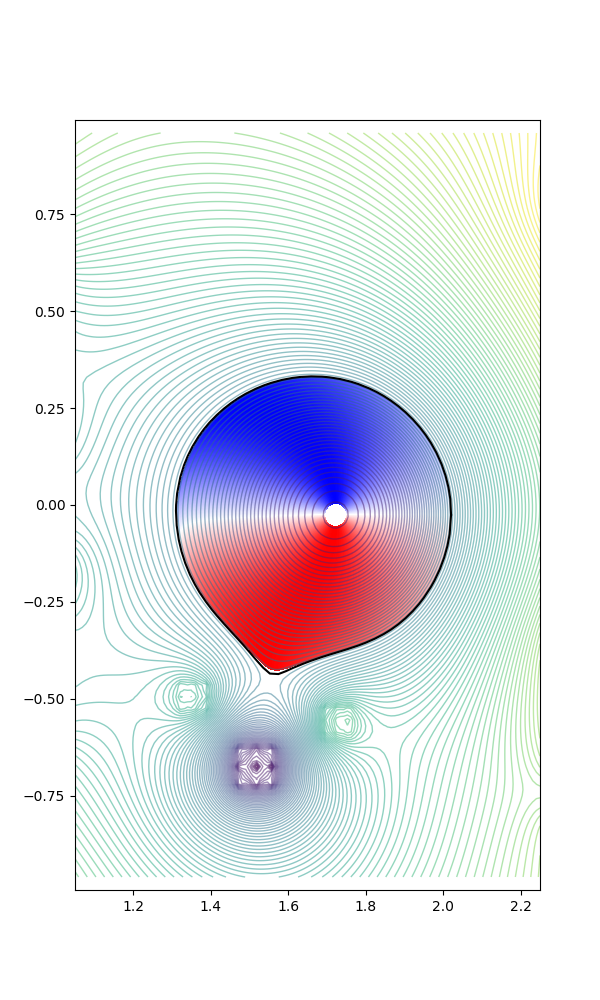
\includegraphics[width=0.15\textwidth]{../psi-code/test_06/test_06_01.png} 
%	}
%	\subfigure{
%		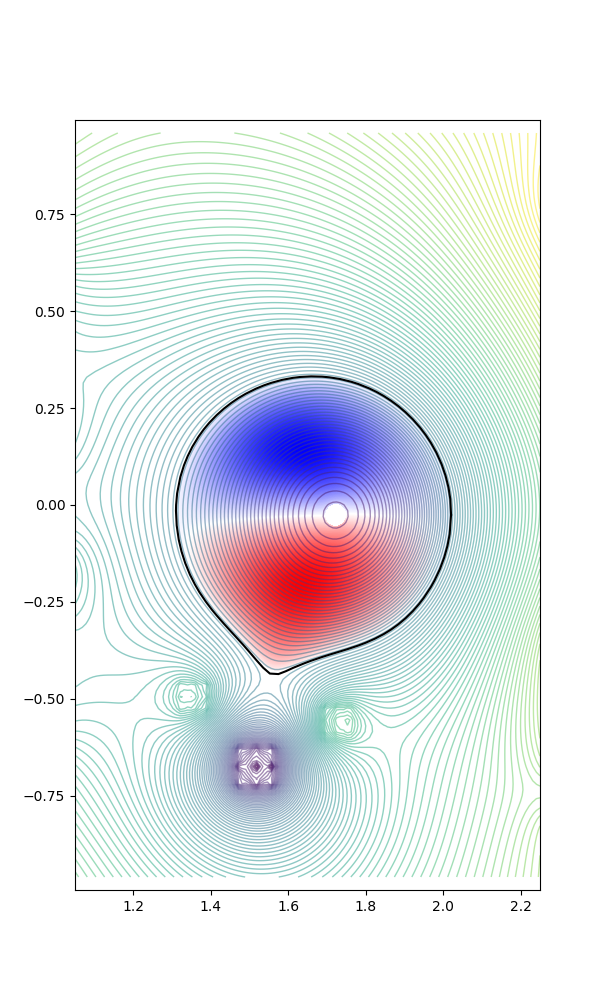
\includegraphics[width=0.15\textwidth]{../psi-code/test_06/test_06_02.png}
%	}
%	\caption{}
%\end{figure}

\section{圆截面近似平衡设置}

这里设置一个圆截面的平衡,主要用来近似小柱坐标系下的情况,将$\psi$设为$r$,选择equal are length的情况,所以$\theta$等同于极向角。方便起见,无量纲坐标分量用$(\psi,\theta,\phi)$和$(r,\theta,\zeta)$表示,带量纲的小半径用$r$表示

\begin{enumerate}
 	\item 设定一个q剖面,这里是一个global的剖面,剖面与小柱坐标系下相同,程序中真正的q剖面为其相反数
 	\item 得到$\Psi$和$Psi'$
 		$$\Psi = \int \frac{rB_0}{qR_0} dr $$ 
 		$$\Psi' = \frac{arB_0}{qR_0}  $$
	\item 坐标的微分量 
		$$ R_\psi = a\cos\theta, R_\theta = -r\sin\theta $$
		$$ Z_\psi = a\sin\theta, Z_\theta =  r\cos\theta $$
	\item 计算雅克比
		$$ J = R(R_\theta Z_\psi - R_\psi Z_\theta) $$
		实际为
		$$ J = -arR $$
	\item 计算度量张量
		$$ |\nabla\psi| = 1/a, |\nabla\theta| = 1/r, \nabla\theta\cdot\nabla\psi = 0 $$ 
	\item q剖面
		$$ q_{local} = -\frac{gJ}{\Psi'R^2} $$
		$$ q_{global} = 

\end{enumerate}


%\section{三场圆截面}
%实际上径向坐标用归一化小半径代替,以下为一些参数设置
%\begin{itemize}
%	\item 环向磁场,$ g = -B_0R_0 $,环向磁场沿着$-\nabla\phi$用来和原始的$(r,\theta,\zeta)$进行对比。
%	\item 极向磁场,$ \Psi = \int{ rB_0/q_{tmp} dr}, \Psi' = arB_0/q_{tmp} $ ,沿着$\theta$正方向。
%	\item 度量分量,$ R_\psi = a\cos\theta $, $ R_\theta = -ar\sin\theta $, $ Z_\psi = a\sin\theta $, $ Z_\theta = ar\sin\theta $
%	\item 雅克比, $ J = R( R_\theta Z_\psi-R_\psi Z_\theta ) $
%	\item $q_{local}$, $ q(\psi,\theta) = -\frac{gJ}{R^2 \Psi} $
%	\item $q_{global}$, $ q_{global} = -\frac{1}{2\pi}\frac{g}{\Psi'}\int_{0}^{2\pi}\frac{J}{R^2}d\theta $, $q_{local}$的极向平均,左手系下和$q_{tmp}$相反
%\end{itemize}
%
%小柱坐标系下圆截面相当于磁面坐标下equal arc length的情况,这时$q_{local}$并不只是$\psi$的函数,小柱坐标系下进行了近似。
%
%\begin{figure}[H]
%	\centering
%	\subfigure[$J$]{
%		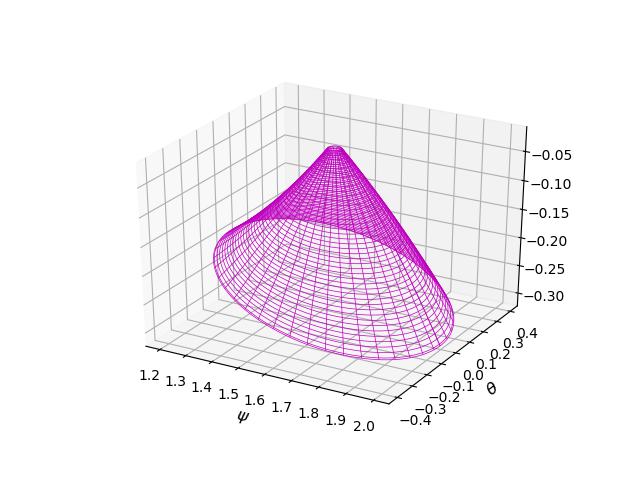
\includegraphics[width=0.2\textwidth]{../psi-code/f2d/jacob.png} 
%	}
%	\subfigure[$q_{local}$]{
%		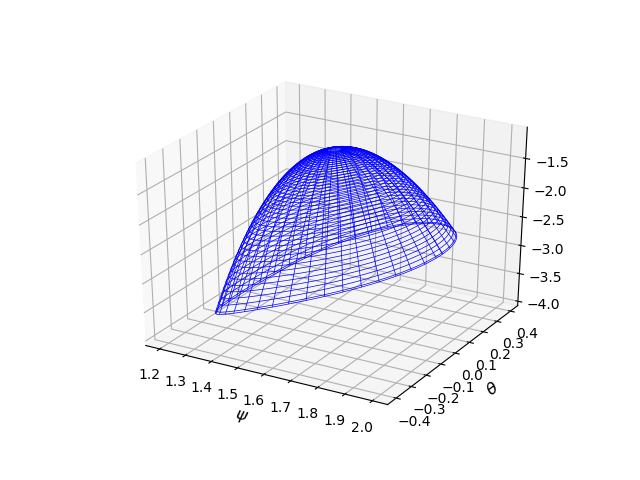
\includegraphics[width=0.2\textwidth]{../psi-code/f2d/q_local.png}
%	}
%	\subfigure[对流项系数$\sim 1/r$]{
%		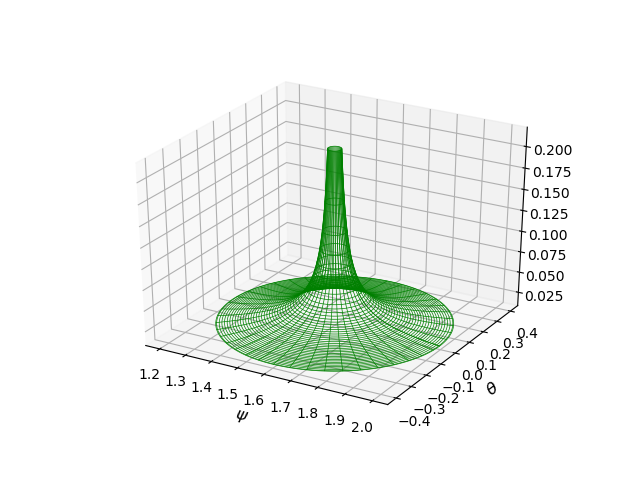
\includegraphics[width=0.2\textwidth]{../psi-code/f2d/coef_con_a.png} 
%	}
%	\subfigure[曲率项系数]{
%		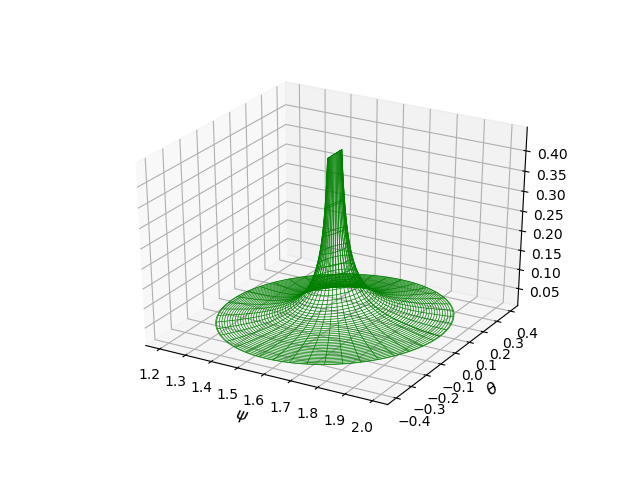
\includegraphics[width=0.2\textwidth]{../psi-code/f2d/coef_cur_a.png} 
%	}
%	\caption{平衡常量对比}
%\end{figure}
%
%以下是相同矩阵的各种项的解,计算的差异主要来自于平行算符归一化时候出现的环径比因子,这个因子在小柱坐标系中是近似而来的,这里全部的微分算符采用二阶精度
%\begin{figure}[H]
%	\centering
%	\subfigure[泊松方程的解]{
%		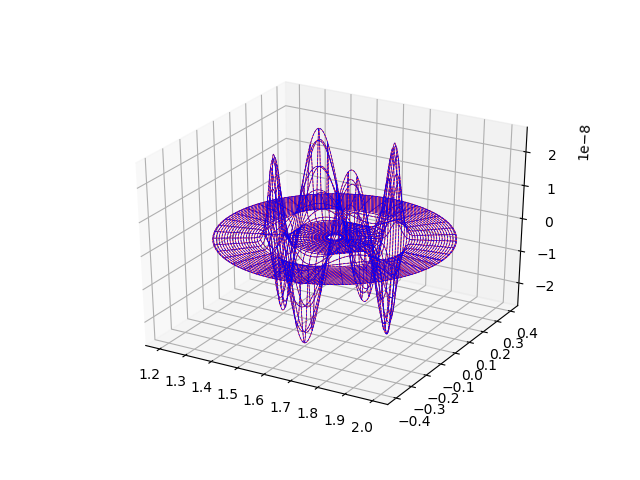
\includegraphics[width=0.2\textwidth]{../psi-code/f2d/test_poisson.png} 
%	}
%	\subfigure[曲率项]{
%		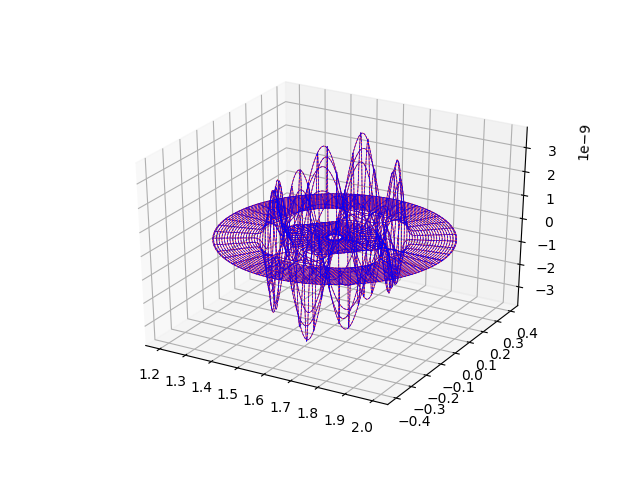
\includegraphics[width=0.2\textwidth]{../psi-code/f2d/test_cur.png}
%	}
%	\subfigure[平行微分项]{
%		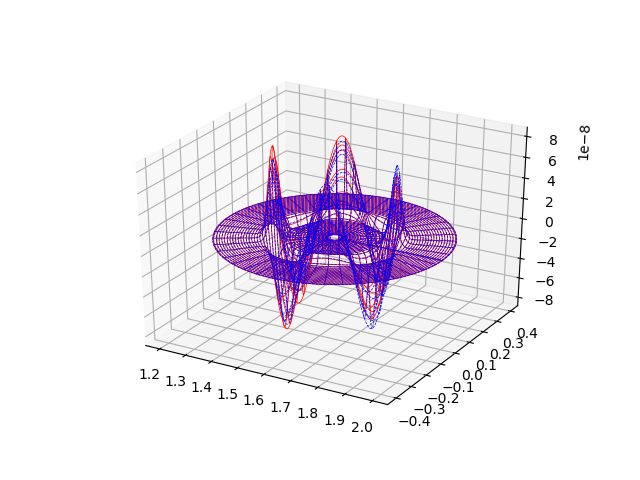
\includegraphics[width=0.2\textwidth]{../psi-code/f2d/test_gradp.png} 
%	}
%	\subfigure[朗道阻尼项]{
%		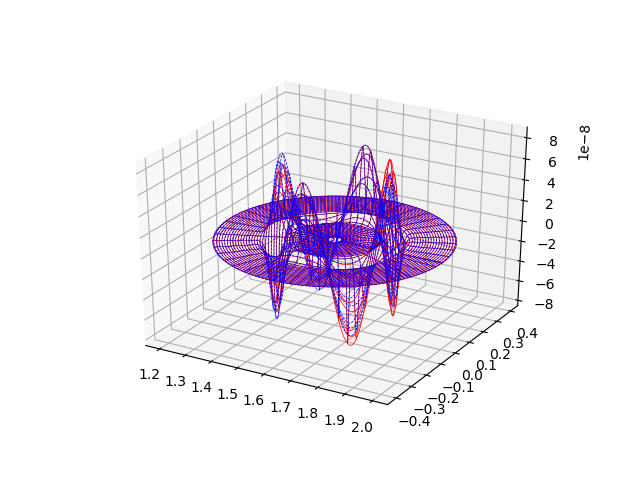
\includegraphics[width=0.2\textwidth]{../psi-code/f2d/test_ld.png} 
%	}
%	\caption{计算变量对比}
%\end{figure}
%
%
%下边主要对比n=10的扰动,平行微分算符有两种表示,分别用$global$和$local$来标记\\
%$(r,\theta,\zeta)$下:
%$$ local: \nabla_{\parallel}{f} = \frac{a}{R}( -f_{\theta}/q_{local}+f_\phi ) $$
%$$ global: \nabla_{\parallel}{f} = \frac{a}{R}(-f_{\theta}/q_{global}+f_\phi ) $$
%这里的$q_{local},q_{global}$均为之前平衡设定下的数值,所以取了相反数
%
%$(\psi,\theta,\phi)$下:
%$$ local: \nabla_{\parallel}{f} = -a\frac{\Psi'}{JB_0}( f_{\theta}+q_{local}f_\phi ) $$
%$$ global: \nabla_{\parallel}{f} = \frac{a}{R}(-f_{\theta}/q_{global}+f_\phi ) $$
%实际上两套坐标系下的表达是一样的。
%
%以下是增长率的对比,实线是小柱坐标,虚线是磁面坐标,两者的差异其实不大,算符基本比较过,可能有一些小的数值没有注意到,这个不是大问题,local的增长率应该取100时刻以后的,之前的模式应该是由于初始扰动的问题。
%\begin{figure}[H]
%	\centering
%	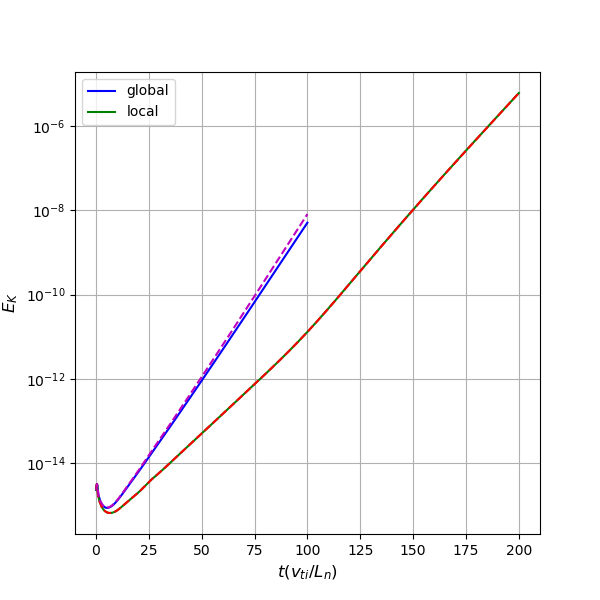
\includegraphics[width=0.35\textwidth]{../psi-code/f2d/E_global_local.png}
%	\caption{}
%\end{figure}
%
%
%\begin{figure}[H]
%	\centering
%	\subfigure[小柱global]{
%		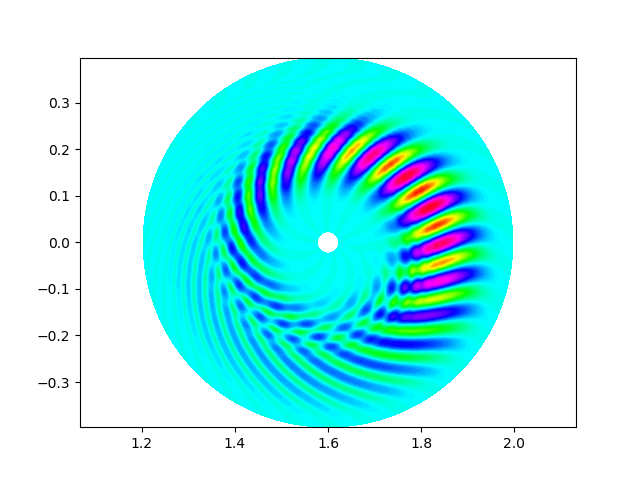
\includegraphics[width=0.2\textwidth]{../psi-code/f2d/test_02_global.png} 
%	}
%	\subfigure[磁面global]{
%		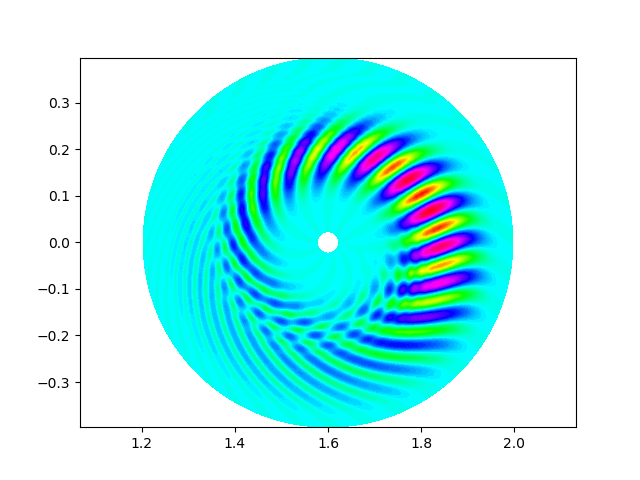
\includegraphics[width=0.2\textwidth]{../psi-code/f2d/test_01_global.png}
%	}
%	\subfigure[小柱local]{
%		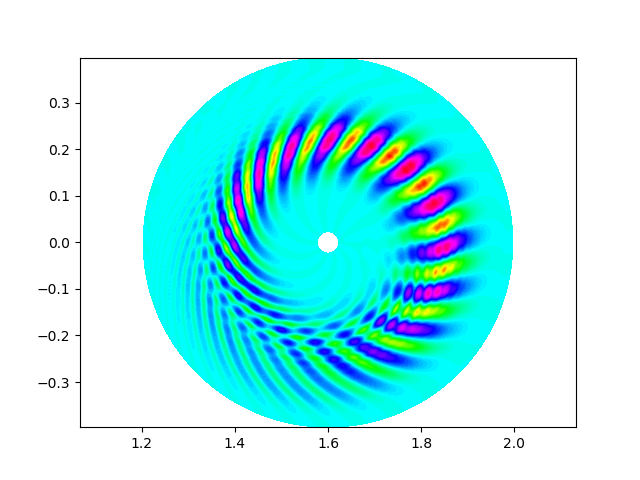
\includegraphics[width=0.2\textwidth]{../psi-code/f2d/test_02_local.png} 
%	}
%	\subfigure[磁面local]{
%		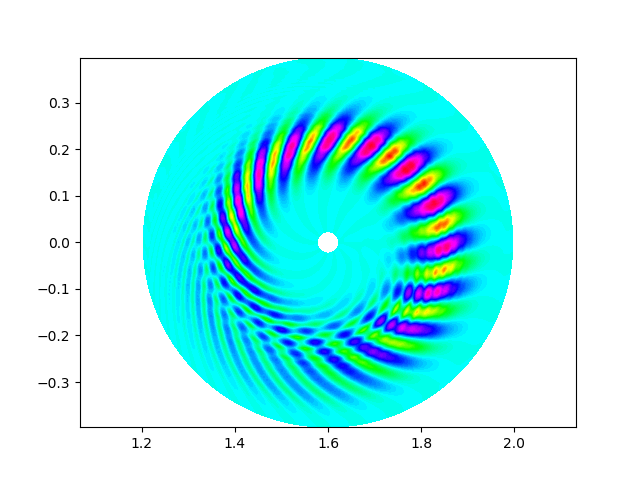
\includegraphics[width=0.2\textwidth]{../psi-code/f2d/test_01_local.png} 
%	}
%	\caption{平衡常量对比}
%\end{figure}
%
%local和global的平行微分算符下增长率有些差别,但是至少说明程序在磁面坐标退化到小柱坐标下的结果应该是合理的。

\end{document}